\chapter{RANDOMNESS AND GRIDLOCK} \label{ch:random}

\epigraph{Everything we care about lies somewhere in the middle, where pattern and randomness interlace.}{James Gleick, \emph{The Information: A History, a Theory, a Flood}}

In this chapter, I define and examine the \emph{gridlock} behavior of the leximin method. In the case of random graphs, I show a reliable tendency that for some edge creation probability $p$, as the network size grows, the occurrence of gridlock becomes more frequent. I show that for any gridlock graph with rational capacities, there exists a constant $k$ such that when the capacities of all edges are $k$, integer flows can be assigned along each path. For diameter-2 random graphs, I conjecture that this value $k$ is $M / [N (N-1) - M]$.





\section{Introduction}

If a community detection method splits a global community into all individuals, and the method has some justification as realistic, then this behavior says that the input is indistinguishable from what random associations would give. Only two levels of structure exist: the macroscopic level of the entire graph and the microscopic level of single nodes. There is no mesoscopic, community structure.

The leximin method for community detection has a tendency to produce the microscopic structure as the only partition in its hierarchy under certain conditions. We call this phenomenon \emph{gridlock}. When it occurs, we affirm that a particular example is \emph{practically} equivalent to random associations. This may suggest that methods which generate hierarchies on these networks lack the causality to do so; instead, they overzealously force communities to be generated in the given example. Obtaining a hierarchy inexplicable by causality is at best problematic and effectively accidental. 

\subsection{Gridlock}

The only replicable partition, irrespective of a random edge creation process, is immediate separation into individual singleton parts. The leximin method can identify such a partition into communities as the only extant one, because every edge is saturated simultaneously. This is \emph{gridlock}. Only the macro- and microscopic structure exist, without a mesoscopic structure. A graph with these properties is called a \emph{gridlock graph}.

What differentiates gridlock from a tie is the width of the stable ranges. In a tie, the stable ranges are tight because ties straddle the boundaries of two behaviors, creating a superposition of dendrogram states. By contrast, gridlock is a stable behavior. The width of the stable range along any axis is not infinitesimally small. Gridlock need not occur at the first level of the hierarchy, but in this work, we specify when gridlock is not immediate. In general, we use the term to refer to immediate gridlock.

A useful lemma about gridlock and modularity can be proven based on a lemma given by Brandes et al.~\cite{brandes2007finding}:
\begin{lemma}
\label{lemma:modularity}

A clustering with maximum modularity has no cluster that consists of a single node with degree 1.
\end{lemma}

Gridlock is a clustering with very low modularity, according to Lemma \autoref{lemma:modularity}. In fact, the modularity of singleton clustering is the minimum possible~\cite{brandes2008modularity}. This suggests a corresponding Lemma:

\begin{lemma}
\label{lemma:grids}

If the modularity-maximizing flat clustering produced by the leximin method is into singletons, then gridlock has occurred. 
\end{lemma}

\begin{proof}
According to Lemma \autoref{lemma:grids}, the singletons of gridlock produce the worst possible modularity. If they are the highest-modularity clustering found, then there exist no other clusterings in the dendrogram. 
\end{proof}

A final observation is that when immediate gridlock occurs, there is only one level in the hierarchy, so the leximin and maximin solutions are the same. Since only one level is solved, rather than up to $N - 1$, a lack of community structure causes the method to \say{fail fast}.



\subsection{Random graphs}

A helpful model to examine this structure of random connections is the binomial graph model. It produces a graph~$G(N, p)$, specifying the number of nodes~$N$ and the probability of an edge between each pair of nodes~$p$. The model was introduced by Gilbert~\cite{gilbert1959random} and analyzed by Erd\H{o}s and R\'enyi~\cite{erdos1960evolution}. 

Much attention has been given to the problem of a dense community \emph{planted} in an otherwise random graph~\cite{hajek2015computational, arias2013community}. Less attention has been given to the \emph{existential} problem of communities in random graphs---of structure inherent in randomness. An exception to this is what has been called \say{one of the most surprising results in the theory of random graphs}: the identification of a reliable largest clique size for a given $p$~\cite{matula1976largest, palmer1985graphical}. Although the largest clique size is replicable across instances of the random graph with given parameters, the particular set of members is almost certainly not replicable. The issue of determining a well-defined cluster of members that should recur is not affected by this observation. Additional work has been done to identify communities in random graphs by consensus using nondeterministic methods~\cite{campigotto2013power} and to relate community size in random graphs to component size~\cite{lipowski2014generic}.

To assess whether there exists a community structure in random graphs, we use the leximin method. For a sufficiently homogeneous graph, the leximin method exhibits gridlock. As the first and only possible partition, it separates the graph into singletons. This dissection suggests a lack of mesoscopic, community structure in the graph. Computational results presented below support this conclusion.





\section{Experimental Evidence} \label{sec:random_experiment}

\begin{figure}
\centering
\begin{subfigure}[c]{0.48\textwidth}
\centering
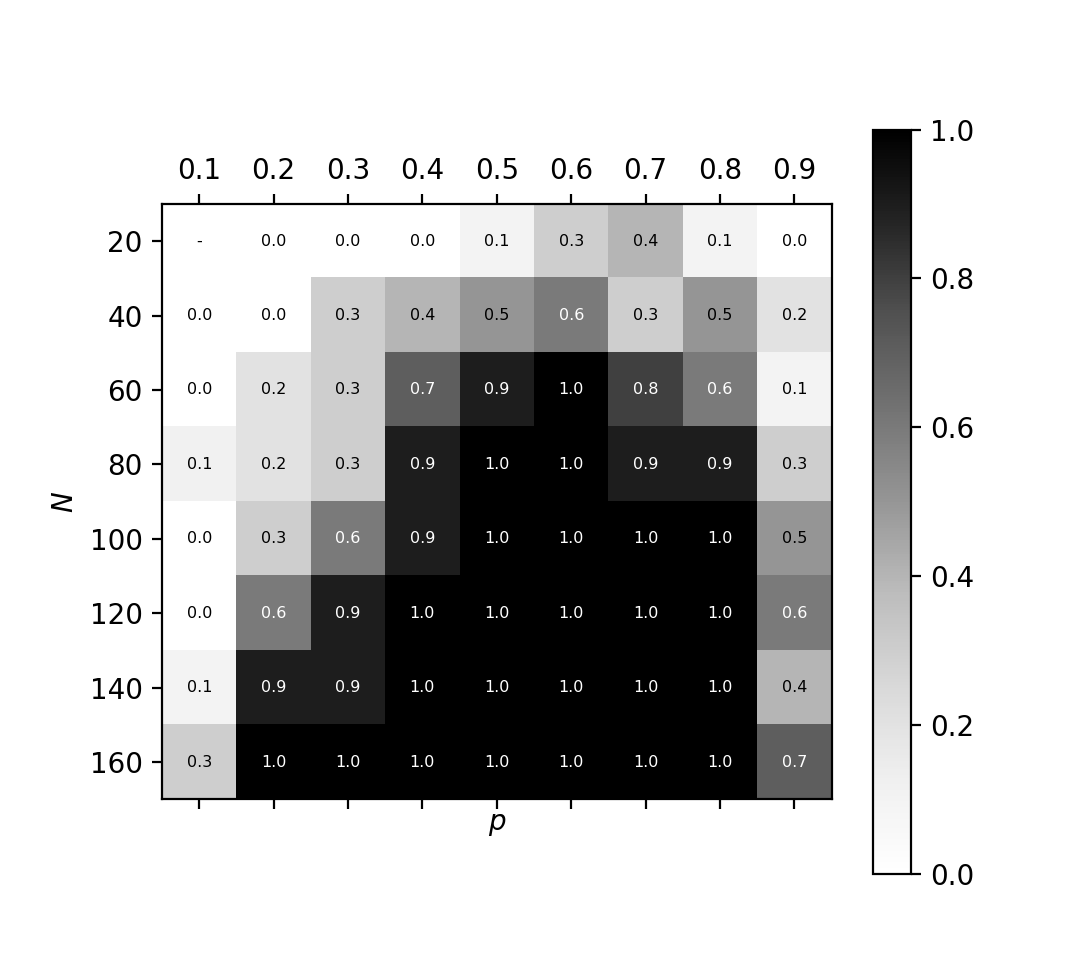
\includegraphics[height=0.225\textheight]{fig/gridlock_big}
\caption{Group 1: 10 trials each}
\end{subfigure}
\quad
\begin{subfigure}[c]{0.48\textwidth}
\centering
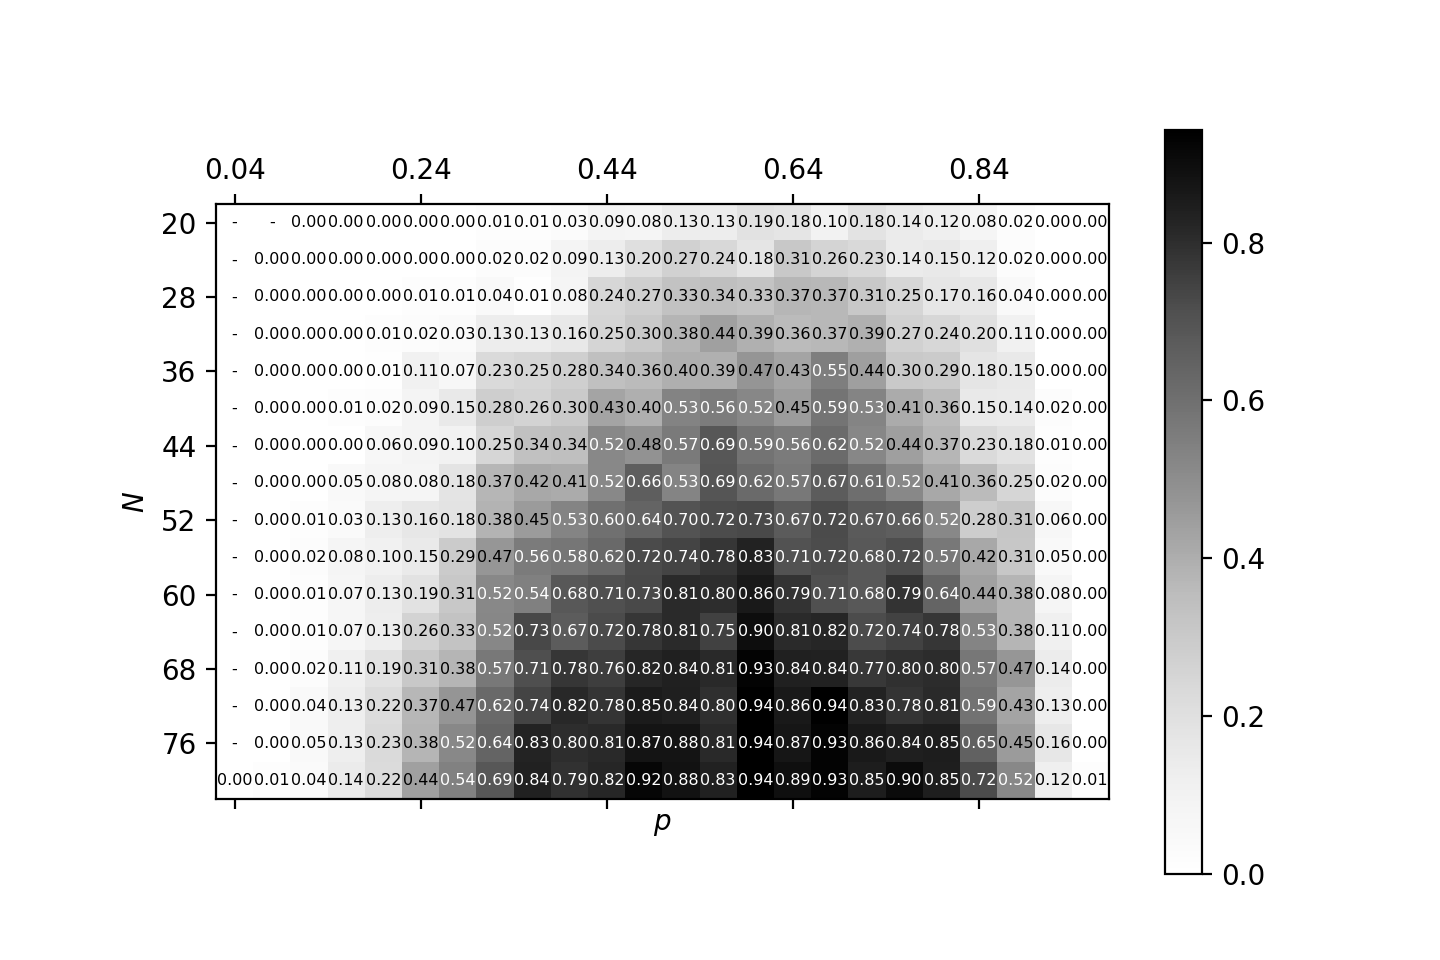
\includegraphics[height=0.225\textheight]{fig/gridlock_small}
\caption{Group 2: 100 trials each}
\end{subfigure}
\caption{Rate of gridlock for each combination of $N$ and $p$}
\label{fig:gridlock}
\end{figure}

To examine the community structure of random graphs, two groups of test graphs were created:
\begin{description}
\item[Group 1.] 10 graphs each at $N = 20, 40, \ldots, 160$ and $p = \frac{1}{10}, \frac{2}{10}, \ldots, \frac{9}{10}$
\item[Group 2.] 100 graphs each at $N = 20, 24, \ldots, 80$ and $p = \frac{1}{25}, \frac{2}{25}, \ldots, \frac{24}{25}$
\end{description}
For each of these parameter combinations, we computed the fraction which display immediate gridlock. From the empirical results shown in \autoref{fig:gridlock}, we see a tendency that for a given $p$, increasing $N$ reliably increases the rate of immediate gridlock.

It is important to note that middle values of the edge probability~$p$ are capable of producing gridlock at lower sizes~$N$, compared to high or low values. For lower values, the reason is that so few edges naturally impart a structure; after all, there is a threshold $p = 1/n$ for the graph to be connected at all~\cite{frieze2015introduction, janson2011random}. On the higher end, gridlock is less common because removing edges from a complete graph (i.e.\ one with $p=1$) produces nodes of minimum degree less than $N - 1$. The resulting asymmetry of node degree generally yields more than one level in the leximin hierarchy. This investigation of the number of levels and the causes is worthy of more investigation.





\section{Discussion}

We can show a result for maximum concurrent flow similar to Menger's theorem for maximum flow~\cite{menger1927allgemeinen}: that a multigraph of the gridlocked graph exists where all edges can be partitioned into edge-disjoint paths with the same number of paths between each node pair.

\begin{theorem}{Edge-disjoint paths in gridlock graphs.} \label{thm:edge}


A multigraph of the gridlocked graph exists where all edges can be partitioned into edge-disjoint paths with the same number of paths between each node pair.
\end{theorem}
\begin{proof}
In a gridlock graph, the demand between all pairs is equal, and the utilized capacity of each edge is equal. The flow may be diverted between various intermediate nodes before reaching its destination, possibly taking multiple paths.

Linear programs with integer coefficients (like the HMCFP) produce rational results~\cite{adler1992polynomial}, so the flow assigned to each path will be rational: a value $p/q$ where $q \ne 0$. Let $k$ be the least common multiple (LCM) of all the denominators of the flows on each path. Assigning this value as the capacity of each edge creates integer-valued flow along all paths, indicating the number of copies of each path. This also means that the capacity of an edge is split into integral flows, from each path that uses that edge.

Each capacitated (weighted) edge with capacity $C$ can be replaced with $C$ unweighted edges, producing the desired multigraph. A path that requires $c < C$ units of flow can utilize $c$ of the $C$ edges. All paths will do this, resulting in edge-disjoint paths on the multigraph. 
\end{proof}

An example application of this theorem is the smallest nontrivial graph with gridlock: $K_{3,2}$. Its throughput is $z = M/[N (N -1) - M] = 6/14 = 3/7$. The flow allocations on each path have denominators of 7 or 14. When scaling up all flows by the LCM of these values, we get 14 unweighted paths between each pair. \autoref{fig:k32_integer} shows the unweighted multigraph's edge-disjoint paths.

\begin{figure}
\centering
\begin{subfigure}[c]{0.48\textwidth}
\centering
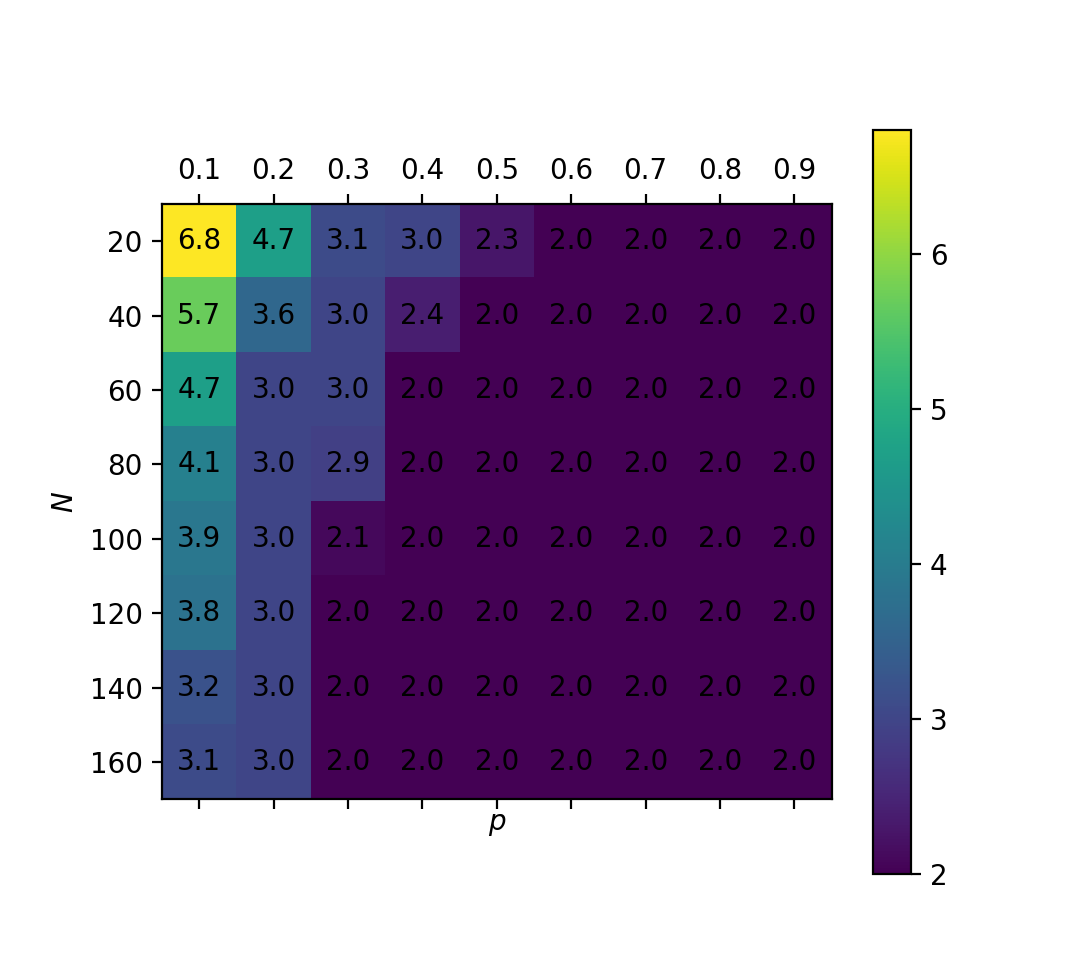
\includegraphics[height=0.225\textheight]{fig/diameter_big}
\caption{Group 1: 10 trials each}
\end{subfigure}
\quad
\begin{subfigure}[c]{0.48\textwidth}
\centering
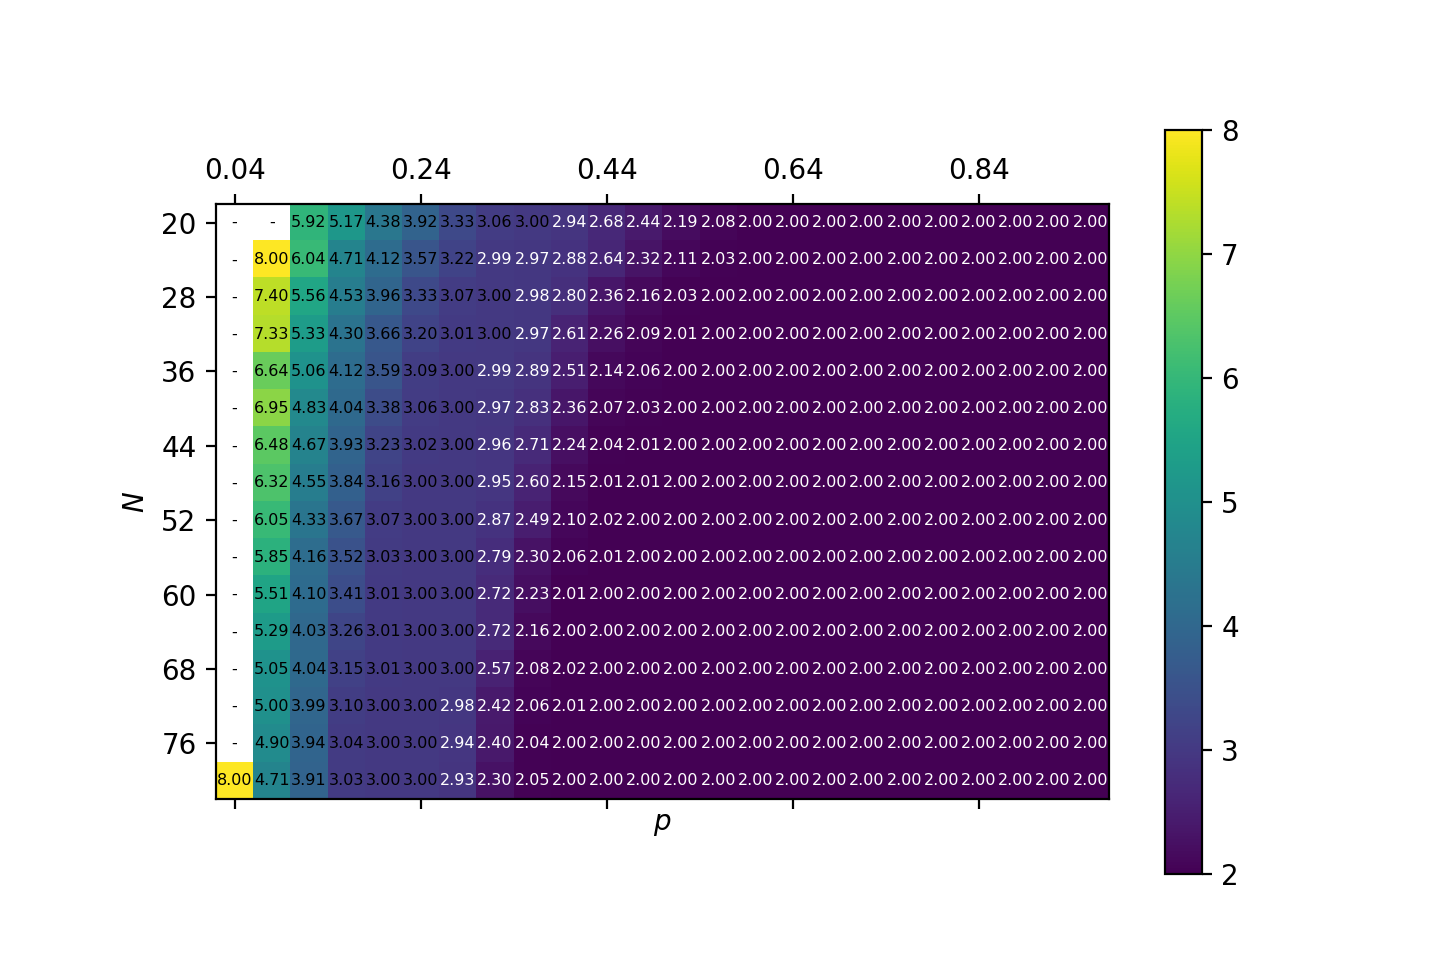
\includegraphics[height=0.225\textheight]{fig/diameter_small}
\caption{Group 2: 100 trials each}
\end{subfigure}
\caption{Average diameter for each combination of $N$ and $p$}
\label{fig:diameter}
\end{figure}

\begin{figure}
\centering
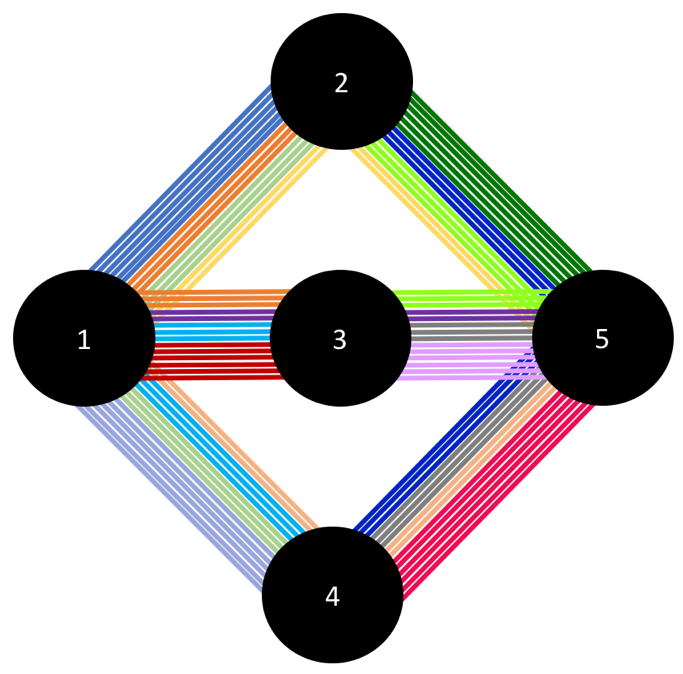
\includegraphics[height=0.25\textheight]{fig/k32_integer}
\caption{The gridlock graph $K_{3,2}$ represented as a multigraph. A single color corresponds to a single route. There are $[N (N-1) - M] = 14$ edges between each node, and 6 are used for demand between each pair of nodes. 2 units between the end nodes 1 and 5 are routed through each middle node 2, 3, and 4. 3 units between each pair of middle nodes are routed through each end node.}
\label{fig:k32_integer}
\end{figure}




\subsection{Gridlock Graphs with Diameter 2}

In the experiment from \autoref{sec:random_experiment}, most graphs that gridlock have diameter 2 (see \autoref{fig:diameter}). This is not a requirement; we see from the $(N=160, p=0.3)$ case that gridlock is possible on a diameter-3 graph (see \autoref{fig:diameter}).

In the case that the diameter is 2, the maximum throughput is easily computable. There exist $|D| = {N \choose 2}$ demand pairs, of which $M$ are at distance 1. Thus, the sum of all shortest path lengths is $M + 2(|D| - M) = 2|D| - M$. These shortest paths must carry all flow, or else we waste capacity by taking longer paths~\cite{mann2008extensions}. Additionally, because we assume unit capacity on each edge, the total capacity is $M$. The throughput is then $z = M / [N (N-1) - M]$. This is the \emph{gridlock bound}, first identified by Biswas and Matula~\cite{biswas1986two}. 

Since throughput is the amount of flow between each pair, we can get an integral flow of $M$ units when we scale up the capacity of each edge by the denominator $[N(N-1)-M]$. 

We can consider specific cases of diameter-2 gridlock graphs with low $p$, with scaled-up edge capacity. These tend to produce several paths at integral flow $M$, as well as some paths with either integral or  fractional values that sum to $M$. We know these values are fractional, rather than irrational, because linear programs with integer coefficients produce rational results~\cite{adler1992polynomial}. The question emerges whether there exists an assignment of flow that is not only rational, but also integral.

\begin{description}
\item[Conjecture.] \emph{In a random graph of diameter 2 and $p<0.5$ that exhibits gridlock, there exists an integer assignment of flows to paths when the capacity of edges is equal to $[N ( N - 1 ) - M ]$.}
\end{description}

As a justification for this conjecture, consider the fact that there exists a multiple of $[N ( N - 1 ) - M ]$ where all paths have integer flow. This comes from Theorem \autoref{thm:edge}. Additionally, the case of $K_{3,2}$ did evenly split its flow along integer paths, as shown in \autoref{fig:k32_integer}. What remains is to show that this multiple is in fact exactly $[N ( N - 1 ) - M ]$ in all such cases.

More work is needed here to prove the conjecture provided above, or to otherwise determine how big the edge multiplicity must be, such that it prescribes a partition into paths with the same number of paths between each node pair. A major hindrance is that while a unique set of critical edges exists, there is not necessarily a unique assignment of flow along paths. To guarantee an integer solution (if it exists) is possible using integer linear programming (ILP), which is NP-hard.

